\section{Auswertung}
\label{sec:Auswertung}
\paragraph{Verwendete Hilfsmittel}
Zur Auswertung und zum plotten aller Daten wird Python \cite{python} inklusive der Packages Matplotlib \cite{matplotlib}, Uncertainties \cite{uncertainties}, Scipy \cite{scipy} und Numpy \cite{numpy} verwendet.

\paragraph{Quantitative Auswertung}
Wird die Wurzel des Photostroms gegen die angelegte Bremsspannung aufgetragen (siehe Abbildungen \ref{fig:blau}, \ref{fig:blau2}, \ref{fig:orange}, \ref{fig:gruen}), so sollte im Bereich $U < 0$ ein linearer Verlauf gemäß
\begin{equation}
  f(x) = ax+b
  \label{eqn:lin}
\end{equation}
erkennbar sein. Ein Fit dieser Funktion mit den Werten aus Tab. \ref{tab:orange}, \ref{tab:gruen}, \ref{tab:blau1}, \ref{tab:blau2}, ergibt die Parameter
\begin{align*}
  a_O &= 0.99 \pm 0.12\\
  a_G &= 1.41 \pm 0.12 \\
  a_{B,1} &= 1.00 \pm 0.08 \\
  a_{B,2} &= 0.67 \pm 0.07
\end{align*}
und
\begin{align*}
  b_O &= (0.45 \pm 0.03) \, \sqrt{\si{\nano \ampere}} \\
  b_G &= (0.75 \pm 0.04) \, \sqrt{\si{\nano \ampere}} \\
  b_{B,1} &= (1.01 \pm 0.05) \, \sqrt{\si{\nano \ampere}} \\
  b_{B,2} &= (0.79 \pm 0.06) \, \sqrt{\si{\nano \ampere}}.
\end{align*}

\begin{figure}
  \centering
  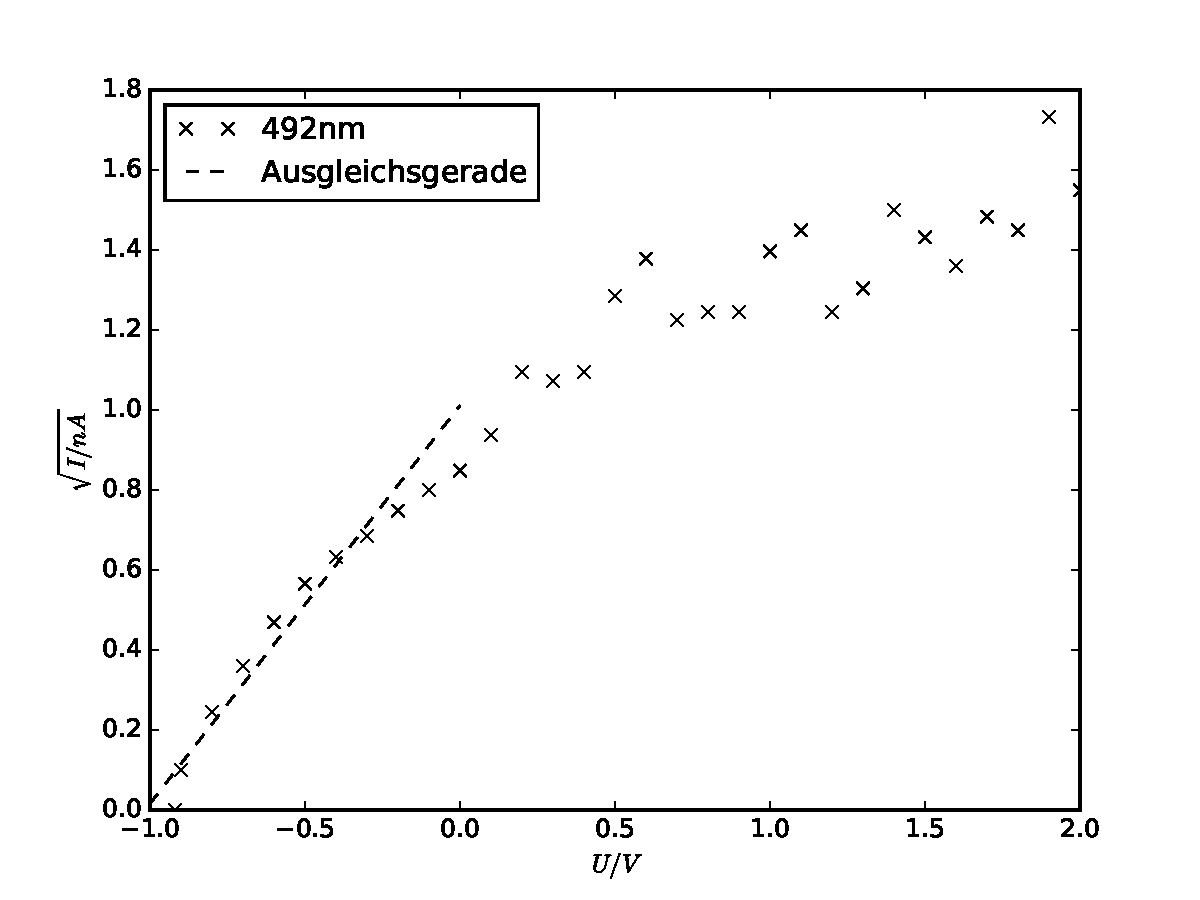
\includegraphics[height = 8cm]{./plots/blau.pdf}
  \caption{Gemessene Spannungen und Ströme der 492nm Spektrallinie.}
  \label{fig:blau}
\end{figure}
\begin{figure}
  \centering
  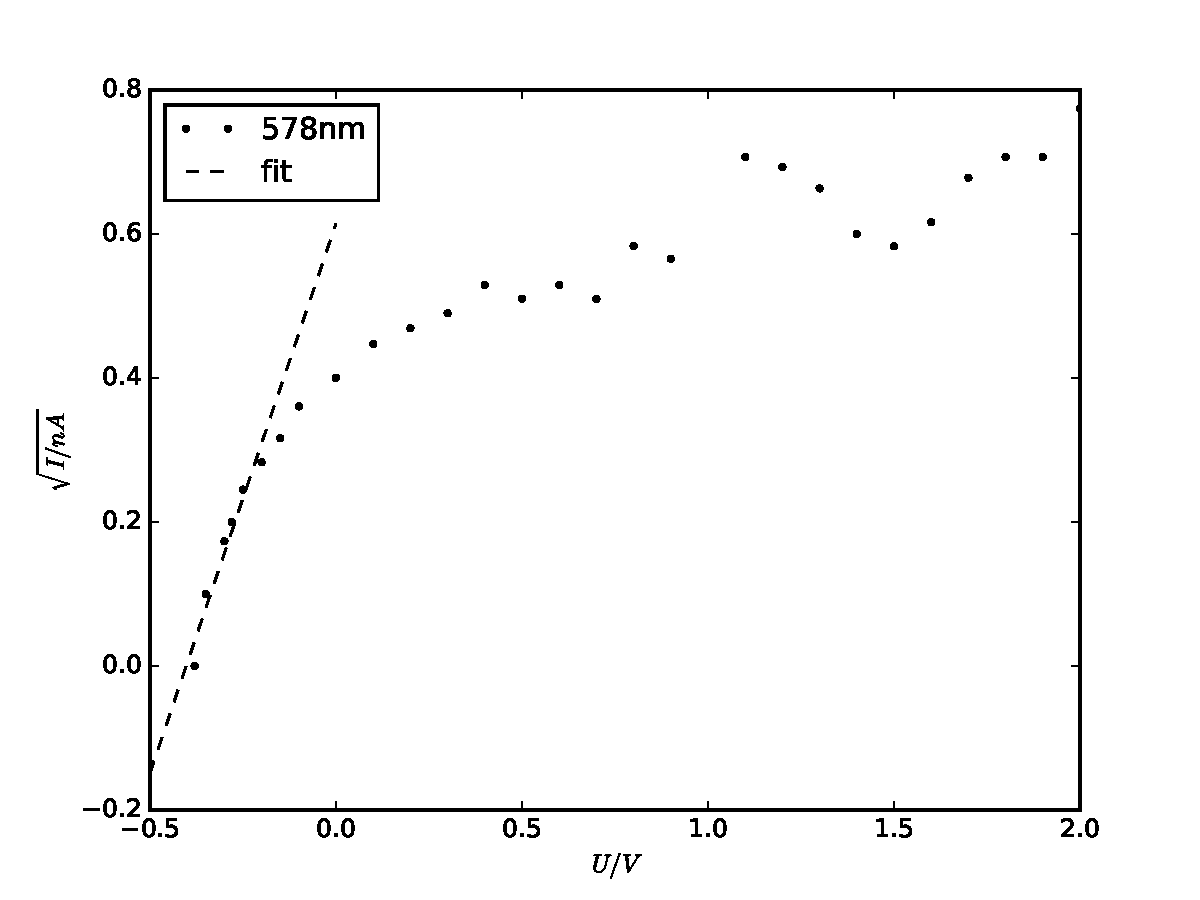
\includegraphics[height = 8cm]{./plots/Orange.pdf}
  \caption{Gemessene Spannungen und Ströme der 578nm Spektrallinie.}
  \label{fig:orange}
\end{figure}
\begin{figure}
  \centering
  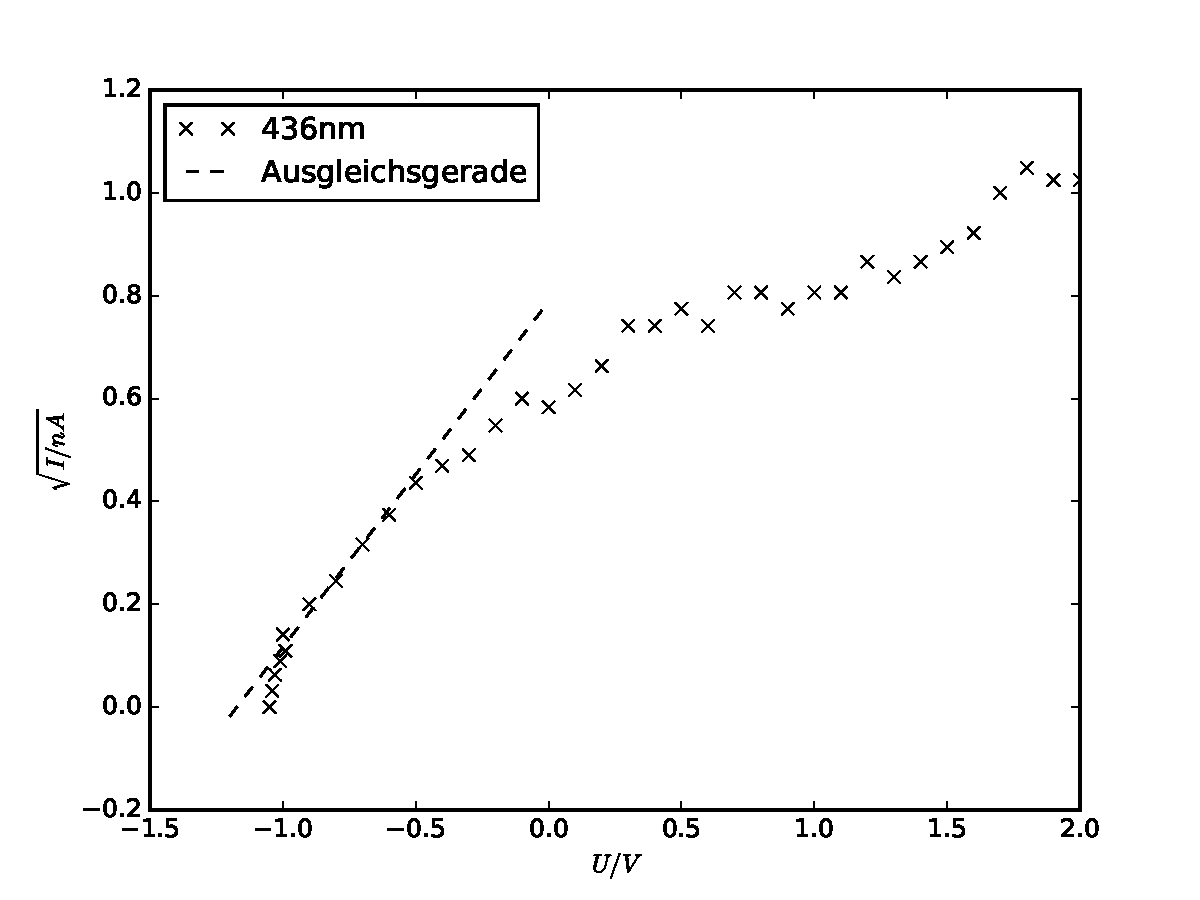
\includegraphics[height = 8cm]{./plots/blau2.pdf}
  \caption{Gemessene Spannungen und Ströme der 436nm Spektrallinie.}
  \label{fig:blau2}
\end{figure}
\begin{figure}
  \centering
  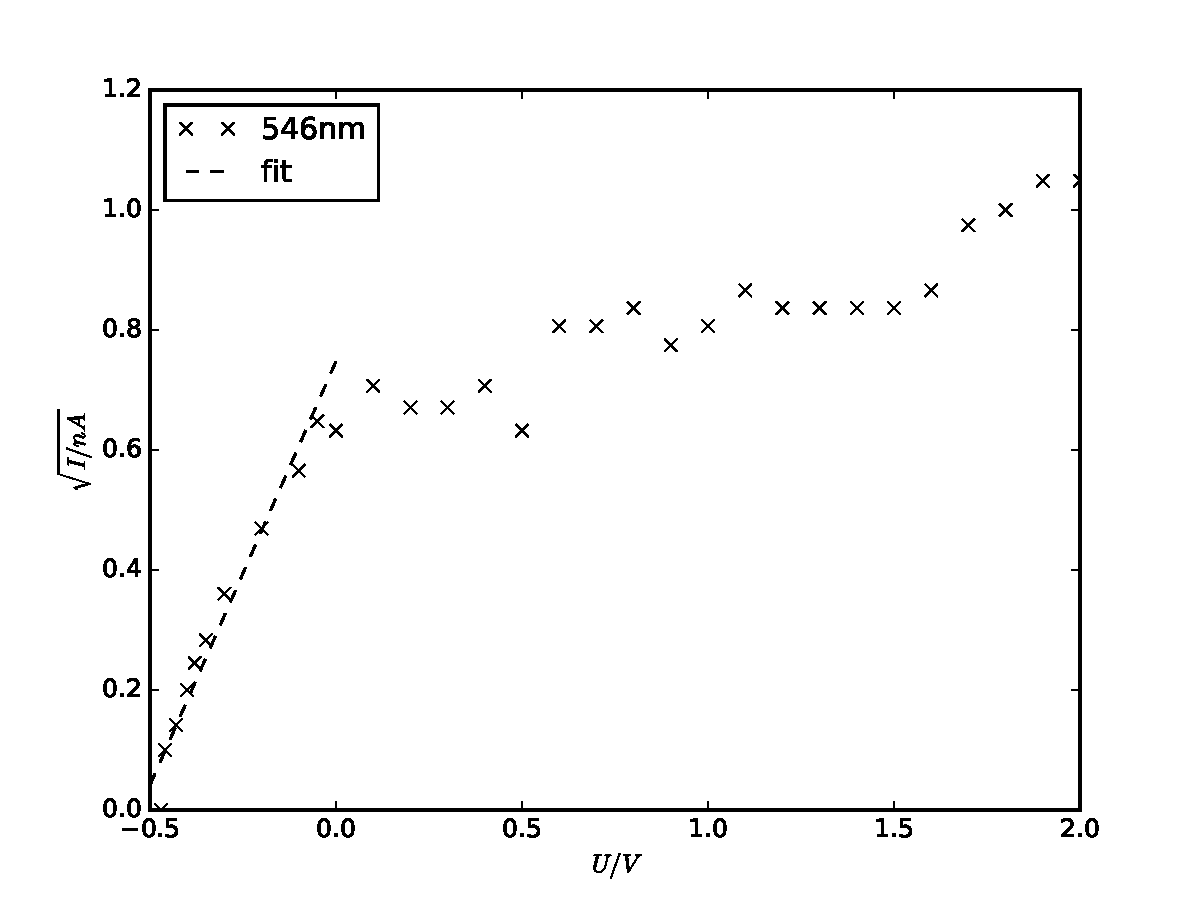
\includegraphics[height = 8cm]{./plots/gruen.pdf}
  \caption{Gemessene Spannungen und Ströme der 546nm Spektrallinie.}
  \label{fig:gruen}
\end{figure}

Berechnung der Nullstellen dieser Ausgleichsgeraden liefert
\begin{align*}
  U_{g,O} &= \SI{-0.45 \pm 0.02}{\volt} \\
  U_{g,G} &= \SI{-0.53 \pm 0.02}{\volt} \\
  U_{g,B,1} &= \SI{-1.01 \pm 0.03}{\volt} \\
  U_{g,B,2} &= \SI{-1.18 \pm 0.05}{\volt}.
\end{align*}

\begin{figure}
  \centering
  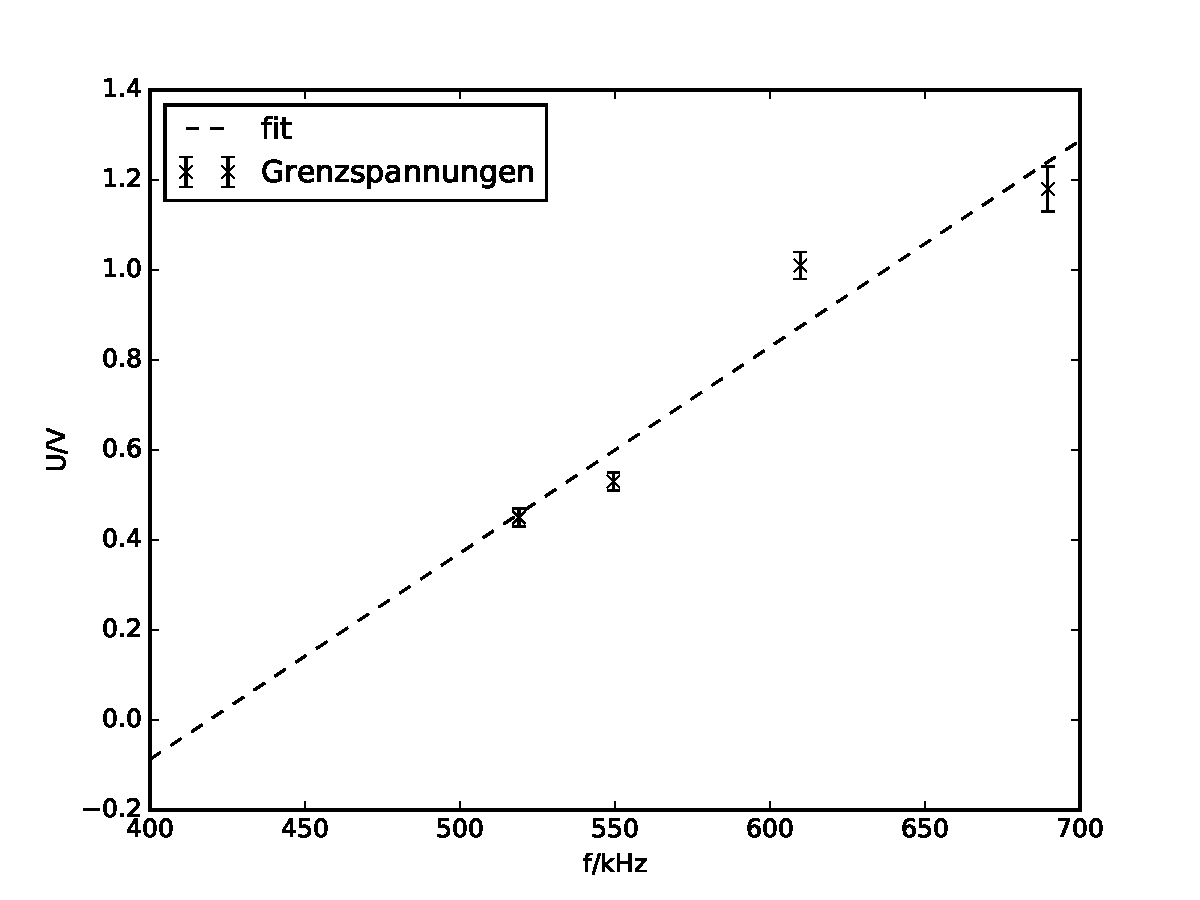
\includegraphics[height = 8cm]{./plots/h.pdf}
  \caption{Grenzspannungen $U_g$ aufgetragen gegen die Frequenz}
  \label{fig:h}
\end{figure}
Diese Werte werden in Abb. \ref{fig:h} aufgetragen und erneut gefittet, um das Plancksche Wirkungsquantum zu bestimmen, wodurch sich die Parameter

\begin{align*}
  a_{h} &= \SI{0.46 \pm 0.09}{\volt \per \kilo \hertz} \\
  b_{h} &= \SI{-1.9 \pm 0.5}{\volt}
\end{align*}
ergeben.
Nach Formel \eqref{eqn:Z} entspricht somit $h/e = a_{h} = \SI{4.6 \pm 0.9}{\femto \volt \second} $.

Man erhält zusätzlich die Austrittsarbeit $A_K$ mit
\begin{equation}
  A_K = b_{h}\cdot e = \SI{1.9 \pm 0.5}{\electronvolt}
\end{equation}


\paragraph{Qualitativer Verlauf des Photostroms}
Der Photostrom der orangenen Kennlinie des Quecksilber ist detaillierter gemessen ind Abb. \ref{fig:fine} dargestellt. Im Bereich der bremsenden Spannung ist der lineare Charakter relativ gut zu erkennen, allerdings lässt sich kein Sättigungsstrom beobachten, welcher sich normalerweise dadurch ergibt, dass alle ausgelösten Elektronen die Anode erreichen.
\begin{figure}
  \centering
  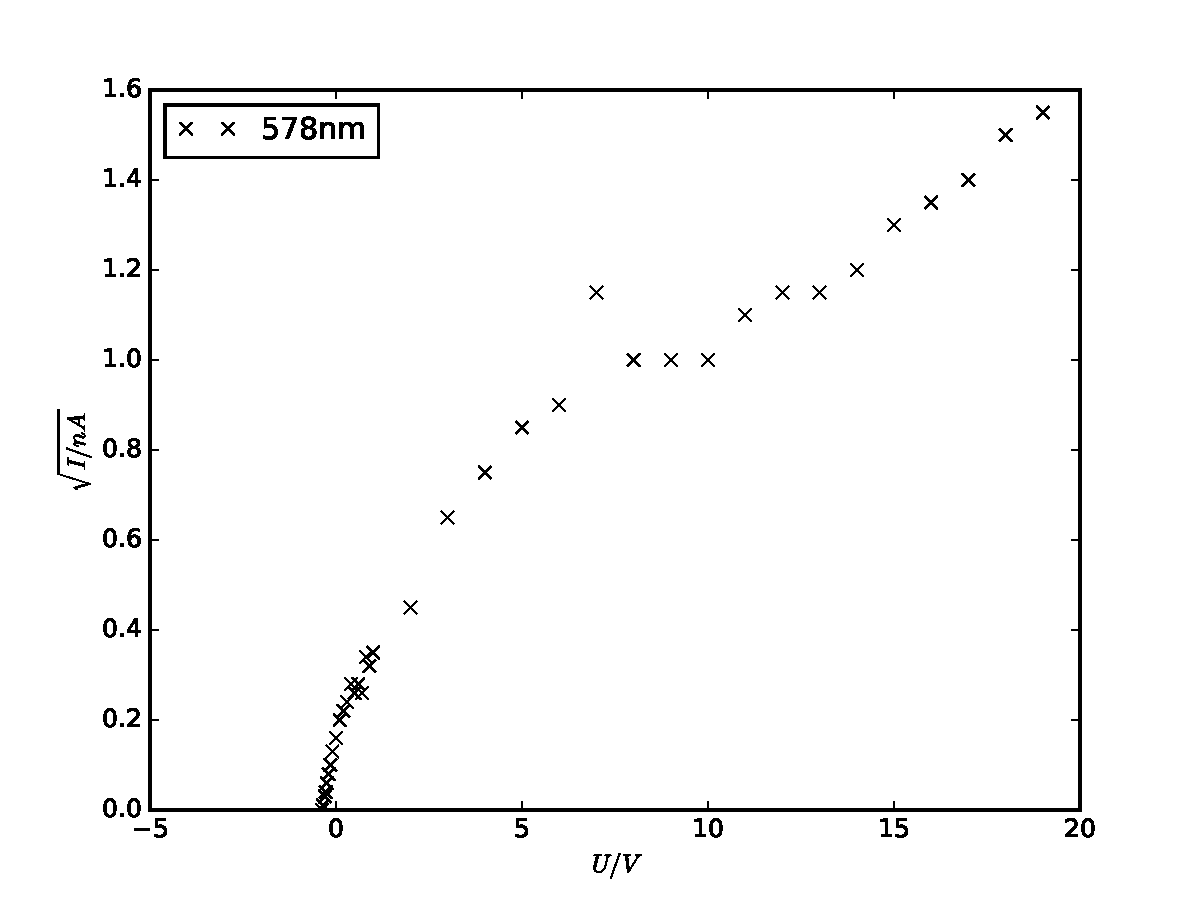
\includegraphics[height = 8cm]{plots/fine.pdf}
  \caption{Gemessener Strom aufgetragen gegen die Bremsspannung bei betrachtung der 578 nm Spektrallinie.}
  \label{fig:fine}
\end{figure}

\paragraph{Tabellen}

\begin{table}
  \centering
  \caption{Messwerte der 578 nm Linie}
  \label{tab:orange}
  \sisetup{round-mode=places}
  \begin{tabular}{S[round-precision = 1]|S[round-precision = 1]}
    \toprule
    $U$/V & $I$/nA \\
    \midrule
    2.000000000000000000e+00 & 5.999999999999999778e-01\\
    1.899999999999999911e+00 & 5.000000000000000000e-01\\
    1.800000000000000044e+00 & 5.000000000000000000e-01\\
    1.699999999999999956e+00 & 4.600000000000000200e-01\\
    1.600000000000000089e+00 & 3.800000000000000044e-01\\
    1.500000000000000000e+00 & 3.400000000000000244e-01\\
    1.399999999999999911e+00 & 3.599999999999999867e-01\\
    1.300000000000000044e+00 & 4.400000000000000022e-01\\
    1.199999999999999956e+00 & 4.799999999999999822e-01\\
    1.100000000000000089e+00 & 5.000000000000000000e-01\\
    9.000000000000000222e-01 & 3.200000000000000067e-01\\
    8.000000000000000444e-01 & 3.400000000000000244e-01\\
    6.999999999999999556e-01 & 2.600000000000000089e-01\\
    5.999999999999999778e-01 & 2.800000000000000266e-01\\
    5.000000000000000000e-01 & 2.600000000000000089e-01\\
    4.000000000000000222e-01 & 2.800000000000000266e-01\\
    2.999999999999999889e-01 & 2.399999999999999911e-01\\
    2.000000000000000111e-01 & 2.200000000000000011e-01\\
    1.000000000000000056e-01 & 2.000000000000000111e-01\\
    -0.000000000000000000e+00 & 1.600000000000000033e-01\\
    -1.000000000000000056e-01 & 1.300000000000000044e-01\\
    -1.499999999999999944e-01 & 1.000000000000000056e-01\\
    -2.000000000000000111e-01 & 8.000000000000000167e-02\\
    -2.500000000000000000e-01 & 5.999999999999999778e-02\\
    -2.800000000000000266e-01 & 4.000000000000000083e-02\\
    -2.999999999999999889e-01 & 2.999999999999999889e-02\\
    -3.499999999999999778e-01 & 1.000000000000000021e-02\\
    -3.800000000000000044e-01 & 0.000000000000000000e+00\\
    \bottomrule
  \end{tabular}
\end{table}

  \begin{table}
    \centering
    \caption{Messwerte der 546 nm Linie}
    \label{tab:gruen}
    \sisetup{round-mode=places}
    \begin{tabular}{S[round-precision = 1]|S[round-precision = 1]}
      \toprule
      $U$/V & $I$/nA \\
      \midrule
      2.000000000000000000e+00 & 1.100000000000000089e+00\\
      1.899999999999999911e+00 & 1.100000000000000089e+00\\
      1.800000000000000044e+00 & 1.000000000000000000e+00\\
      1.699999999999999956e+00 & 9.499999999999999556e-01\\
      1.600000000000000089e+00 & 7.500000000000000000e-01\\
      1.500000000000000000e+00 & 6.999999999999999556e-01\\
      1.399999999999999911e+00 & 6.999999999999999556e-01\\
      1.300000000000000044e+00 & 6.999999999999999556e-01\\
      1.199999999999999956e+00 & 6.999999999999999556e-01\\
      1.100000000000000089e+00 & 7.500000000000000000e-01\\
      1.000000000000000000e+00 & 6.500000000000000222e-01\\
      9.000000000000000222e-01 & 5.999999999999999778e-01\\
      8.000000000000000444e-01 & 6.999999999999999556e-01\\
      6.999999999999999556e-01 & 6.500000000000000222e-01\\
      5.999999999999999778e-01 & 6.500000000000000222e-01\\
      5.000000000000000000e-01 & 4.000000000000000222e-01\\
      4.000000000000000222e-01 & 5.000000000000000000e-01\\
      2.999999999999999889e-01 & 4.500000000000000111e-01\\
      2.000000000000000111e-01 & 4.500000000000000111e-01\\
      1.000000000000000056e-01 & 5.000000000000000000e-01\\
      -0.000000000000000000e+00 & 4.000000000000000222e-01\\
      -5.000000000000000278e-02 & 4.199999999999999845e-01\\
      -1.000000000000000056e-01 & 3.200000000000000067e-01\\
      -2.000000000000000111e-01 & 2.200000000000000011e-01\\
      -2.999999999999999889e-01 & 1.300000000000000044e-01\\
      -3.499999999999999778e-01 & 8.000000000000000167e-02\\
      -3.800000000000000044e-01 & 5.999999999999999778e-02\\
      -4.000000000000000222e-01 & 4.000000000000000083e-02\\
      -4.299999999999999933e-01 & 2.000000000000000042e-02\\
      -4.600000000000000200e-01 & 1.000000000000000021e-02\\
      -4.699999999999999734e-01 & 0.000000000000000000e+00\\
      \bottomrule
    \end{tabular}
\end{table}

\begin{table}
  \centering
  \caption{Messwerte der 492nm Linie}
  \label{tab:blau1}
  \sisetup{round-mode=places}
  \begin{tabular}{S[round-precision = 1]|S[round-precision = 1]}
    \toprule
    $U$/V & $I$/nA \\
    \midrule
    2.000000000000000000e+00 & 2.399999999999999911e+00\\
    1.899999999999999911e+00 & 3.000000000000000000e+00\\
    1.800000000000000044e+00 & 2.100000000000000089e+00\\
    1.699999999999999956e+00 & 2.200000000000000178e+00\\
    1.600000000000000089e+00 & 1.850000000000000089e+00\\
    1.500000000000000000e+00 & 2.049999999999999822e+00\\
    1.399999999999999911e+00 & 2.250000000000000000e+00\\
    1.300000000000000044e+00 & 1.699999999999999956e+00\\
    1.199999999999999956e+00 & 1.550000000000000044e+00\\
    1.100000000000000089e+00 & 2.100000000000000089e+00\\
    1.000000000000000000e+00 & 1.949999999999999956e+00\\
    9.000000000000000222e-01 & 1.550000000000000044e+00\\
    8.000000000000000444e-01 & 1.550000000000000044e+00\\
    6.999999999999999556e-01 & 1.500000000000000000e+00\\
    5.999999999999999778e-01 & 1.899999999999999911e+00\\
    5.000000000000000000e-01 & 1.649999999999999911e+00\\
    4.000000000000000222e-01 & 1.199999999999999956e+00\\
    2.999999999999999889e-01 & 1.149999999999999911e+00\\
    2.000000000000000111e-01 & 1.199999999999999956e+00\\
    1.000000000000000056e-01 & 8.800000000000000044e-01\\
    -0.000000000000000000e+00 & 7.199999999999999734e-01\\
    -1.000000000000000056e-01 & 6.400000000000000133e-01\\
    -2.000000000000000111e-01 & 5.600000000000000533e-01\\
    -2.999999999999999889e-01 & 4.699999999999999734e-01\\
    -4.000000000000000222e-01 & 4.000000000000000222e-01\\
    -5.000000000000000000e-01 & 3.200000000000000067e-01\\
    -5.999999999999999778e-01 & 2.200000000000000011e-01\\
    -6.999999999999999556e-01 & 1.300000000000000044e-01\\
    -8.000000000000000444e-01 & 5.999999999999999778e-02\\
    -9.000000000000000222e-01 & 1.000000000000000021e-02\\
    -9.200000000000000400e-01 & 0.000000000000000000e+00\\
    \bottomrule
  \end{tabular}
\end{table}

\begin{table}
  \centering
  \caption{Messwerte der 436nm Linie}
  \label{tab:blau2}
  \sisetup{round-mode=places}
  \begin{tabular}{S[round-precision = 1]|S[round-precision = 1]}
    \toprule
    $U$/V & $I$/nA \\
    \midrule
    2.000000000000000000e+00 & 1.050000000000000044e+00\\
    1.899999999999999911e+00 & 1.050000000000000044e+00\\
    1.800000000000000044e+00 & 1.100000000000000089e+00\\
    1.699999999999999956e+00 & 1.000000000000000000e+00\\
    1.600000000000000089e+00 & 8.499999999999999778e-01\\
    1.500000000000000000e+00 & 8.000000000000000444e-01\\
    1.399999999999999911e+00 & 7.500000000000000000e-01\\
    1.300000000000000044e+00 & 6.999999999999999556e-01\\
    1.199999999999999956e+00 & 7.500000000000000000e-01\\
    1.100000000000000089e+00 & 6.500000000000000222e-01\\
    1.000000000000000000e+00 & 6.500000000000000222e-01\\
    9.000000000000000222e-01 & 5.999999999999999778e-01\\
    8.000000000000000444e-01 & 6.500000000000000222e-01\\
    6.999999999999999556e-01 & 6.500000000000000222e-01\\
    5.999999999999999778e-01 & 5.500000000000000444e-01\\
    5.000000000000000000e-01 & 5.999999999999999778e-01\\
    4.000000000000000222e-01 & 5.500000000000000444e-01\\
    2.999999999999999889e-01 & 5.500000000000000444e-01\\
    2.000000000000000111e-01 & 4.400000000000000022e-01\\
    1.000000000000000056e-01 & 3.800000000000000044e-01\\
    -0.000000000000000000e+00 & 3.400000000000000244e-01\\
    -1.000000000000000056e-01 & 3.599999999999999867e-01\\
    -2.000000000000000111e-01 & 2.999999999999999889e-01\\
    -2.999999999999999889e-01 & 2.399999999999999911e-01\\
    -4.000000000000000222e-01 & 2.200000000000000011e-01\\
    -5.000000000000000000e-01 & 1.900000000000000022e-01\\
    -5.999999999999999778e-01 & 1.400000000000000133e-01\\
    -6.999999999999999556e-01 & 1.000000000000000056e-01\\
    -8.000000000000000444e-01 & 5.999999999999999778e-02\\
    -9.000000000000000222e-01 & 4.000000000000000083e-02\\
    -9.899999999999999911e-01 & 1.200000000000000025e-02\\
    -1.000000000000000000e+00 & 2.000000000000000042e-02\\
    -1.010000000000000009e+00 & 8.000000000000000167e-03\\
    -1.030000000000000027e+00 & 4.000000000000000083e-03\\
    -1.040000000000000036e+00 & 1.000000000000000021e-03\\
    -1.050000000000000044e+00 & 0.000000000000000000e+00\\
    \bottomrule
  \end{tabular}
\end{table}
